
\chapter{Governing equations for free surface flows}
\label{equations}



%Before introducing the review of the numerical methods, the governing equations will be presented.
%The following sections are devoted for the numerical methods.
%The last section is about the coupling algorithms.



%\section{Free surface flows}


Water related natural hazards usually involve free surface flows.
This property allows to assume some simplifications, specially at the large scale.
For this reason, the general case describing the fluid motion is presented first, the Navier-Stokes equations.
Then, some simplifications for the free surface flows are made, yielding the shallow water equations. Different assumptions for the depth integrated models will provide different sets of equations and its range of applicability as well as physical properties will be explained.




\section{Navier-Stokes equations}


The motion of a fluid is described by the Navier-Stokes equations. The case of a free surface flow is described by that equations and the free surface is located where the densities or the fluid properties are discontinuous. In general, an air-water interface is assumed but some natural phenomena may include a more complex configuration, such as debris flow-air-water interfaces. All this continuous media can be considered isotermal and incompressible, and the standard formulation of the Navier-Stokes equations can be used.

The problem consists in the incompressible Navier-Stokes equations in a time interval $(0, t_f)$ and in a spatial domain $\Omega \in \mathbb{R}^{n_d}$, being $n_d$ the number of space dimensions, $3$ unless otherwise stated. Let $t$ be a certain time instant in the temporal domain $(0, t_f)$ and $\mathbf{x}$ a given point in the spatial domain $\Omega$. The balance equations for the momentum and mass are written in the following form:
\begin{subequations} \label{NS}
    \begin{align} \label{NS1}
        \pder{u_i}{t} + u_j \pder{u_i}{x_i} + \frac{1}{\rho} \pder{p}{x_i} +
            \frac{1}{\rho} \pder{}{x_i} \tau_{ij} &= f_i \\ \label{NS2}
        \pder{u_i}{x_i} &= 0
    \end{align}
\end{subequations}
With the appropriate initial and boundary conditions. Let $\Gamma$ be the boundary of the domain $\Omega$ and $\mathbf{n}$ the unit outward normal on $\Gamma$. Dirichlet and Neumann boundary conditions are considered, $\Gamma_D$ and $\Gamma_N$ respectively, such that $\Gamma_D \cup \Gamma_N = \Gamma$.
The usual summation convention is used if there is index repetition.
$\rho$ is the fluid density, $p$ is the pressure, $\mathbf{u}$ is the velocity, $\bm{\tau}$ is the viscous stresses tensor and $\mathbf{f}$ is the body forces vector.




%%%%%%%%%%%%%%%%%%%%%%%%%%%%%%%%%%%%%%%%
%%%%%%%%%%%%%%%%%%%%%%%%%%%%%%%%%%%%%%%%
%%%%%%%%%%%%%%%%%%%%%%%%%%%%%%%%%%%%%%%%




\section{Shallow water equations}


The flow of water in shallow layers occurs in a wide range of situations, such as coastal dynamics and hydraulics. In these free surface flows in relatively thin layers compared to the characteristic horizontal length, the horizontal velocities are of primary importance. Under that circumstances, the problem can be reasonably approximated the horizontal plane.

The shallow water equations are the result of integrating vertically the Navier-Stokes equations, assuming incompressibility, small vertical velocity and negligible vertical acceleration \cite{abbot1979,zien3}. The assumptions over the vertical velocity and its acceleration are equivalent to hydrostatic pressure, in fact, the vertical component of the momentum equation (\ref{NS1}) is reduced to
\begin{equation} \label{SW_hydrostatic_pressure}
    \frac{1}{\rho}\pder{p}{x_3} + g = 0
\end{equation}

After substitution of the hydrostatic pressure assumption \ref{SW_hydrostatic_pressure} into the mass conservation \ref{NS2}, the governing equations are integrated from the bottom $z$ to the free surface $\eta$. The problem is closed by adding two kinematic boundary conditions at the bottom and the free surface:
\begin{equation}
    u_3(\eta) = \frac{D\eta}{Dt} \ , \quad u_3(z) = \frac{Dz}{Dt}
\end{equation}


The governing equations are expressed in terms of a new set of primary variables: the water depth and the horizontal flow rate. The water depth is defined by the integration limits, $h = z + \eta$ and the averaged horizontal flow rate $\mathbf{q}$ is defined by the following integrated value,
\begin{equation} \label{SW_averaged_momentum}
    \mathbf{q} = \int_z^\eta \mathbf{u}\,dx_3
\end{equation}
To avoid introducing extra notation, in a shallow water context, $\mathbf{u}$ refers to the averaged horizontal velocities. In that case, the expression \ref{SW_averaged_momentum} can be reduced to a compact form as $\mathbf{q} = h\mathbf{u}$.


Here we find that the resulting equations are written in the same form as the Euler conservation equations. In spite the equations present some similarities to the compressible flow, the shallow water equations are describing a purely incompressible fluid: the variable water depth is playing the role of the variable pressure in compressible fluids. The equations read
%The equations governing mass and momentum conservation can be written in conservative form with water depth $h$ and specific discharge $\mathbf{q}=(h\mathbf{u})$ as follows,
\begin{equation} \label{general_sw}
\pder{\bm{\phi}}{t} + \pder{\mathbf{F}_i}{x_i} + \pder{\mathbf{G}_i}{x_i} + \mathbf{Q} = \mathbf{0} \qquad \text{for} \enspace i=1,2
\end{equation}
with

\begin{subequations}\label{variables_and_fluxes}
\allowdisplaybreaks
\begin{align}
\bm{\phi} &= \left\{
    \begin{array}{c}
        hu_1 \\
        hu_2 \\
        h
    \end{array}\right\} \\
\mathbf{F}_i &= \left\{
    \begin{array}{c}
        hu_1u_i + \delta_{1i}\frac{1}{2}g(h^2 - z^2) \\ [5pt]
        hu_2u_i + \delta_{2i}\frac{1}{2}g(h^2 - z^2) \\ [5pt]
        hu_i
    \end{array}\right\} \\
\mathbf{G}_i &= \left\{
    \begin{array}{c}
        -(h/\rho) \bar{\tau}_{1i} \\ [5pt]
        -(h/\rho) \bar{\tau}_{2i} \\ [5pt]
        0
    \end{array}\right\} \\
\mathbf{Q} &= \left\{
    \begin{array}{c}
        \displaystyle -g(h-z)\pder{z}{x_1} + \frac{h}{\rho}\pder{p_a}{x_1}
        - \frac{1}{\rho}\tau^s_{31} + \frac{1}{\rho}\tau^b_{31} \\ [10pt]
        \displaystyle -g(h-z)\pder{z}{x_2} + \frac{h}{\rho}\pder{p_a}{x_2}
        - \frac{1}{\rho}\tau^s_{32} + \frac{1}{\rho}\tau^b_{32} \\ [10pt]
        r
    \end{array}\right\}
\end{align}
\end{subequations}
where $\bm{\phi}$ is the vector of conserved variables, $\mathbf{F}_i$ is the vector of convective fluxes, $\mathbf{G}_i$ is the vector of viscous fluxes and $\mathbf{Q}$ is the vector source terms. In Figure \ref{diagram} there is a representation of the variables and the notation. The coordinates are denoted with the index notation $x_i$. Since this formulation is defined in a two dimensional space ($n_d=2$), in the following we will consider $i=1,2$.
$\delta_{ij}$ is the Kronecker delta. The topography is expressed with the variable $z$ and the free surface elevation is expressed in terms of the topography and the total depth, $\eta = z + h$. $\bar{\tau}_{ij}$ are the averaged horizontal stresses, and $\tau^b_{3i}$ and $\tau^s_{3i}$ denote the bottom and surface friction stresses respectively. Finally, $r$ is the rain source term and $p_a$ is the atmospheric pressure.


\begin{figure}
    \centering
    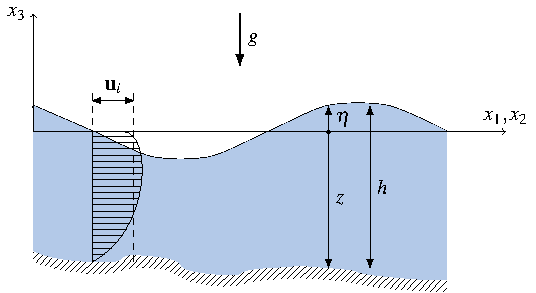
\includegraphics[width=.8\textwidth]{img/eq/diagram.pdf}
    \caption{Diagram and notation for the balance equations (\ref{general_sw}) and (\ref{variables_and_fluxes})}
    \label{diagram}
\end{figure}



Usually, the bottom friction $\tau^b_{3i}$ from (\ref{variables_and_fluxes}) is modelled with a semi-empirical formula, such as the Chezy or the Manning formula. The Manning formula generalized for two dimensions is as follows:
\begin{equation}
\frac{\tau^b_{3i}}{\rho} = -gn^2\frac{\abs{\mathbf{q}}\mathbf{q}}{h^{\sfrac{7}{3}}}
\end{equation}
where $n$ is the Manning roughness coefficient. It defines the resistance to flow by the roughness of the bottom or other macroscopic factors and it is determined empirically. In practice, the Manning coefficient varies from $0.009$ for a very smooth bed (concrete) to $0.05$ for a rough bed (rocks) \cite{chow1988}.


The averaged horizontal stresses are calculated from the combination of the molecular stresses and the Reynolds stresses as follows
\begin{equation} \label{stresses}
\frac{\bar{\tau}_{ij}}{\rho} = (\nu + \nu_t)\left(
    \pder{u_i}{x_j} + \pder{u_j}{x_i} -\frac{2}{3}\delta_{ij}\pder{u_k}{x_k} \right)
\end{equation}
where $\nu$ is the kinematic viscosity and $\nu_t$ is the turbulent kinematic viscosity. When any model of turbulence is considered, the turbulent stresses can be considered as included in the bottom friction with the Manning formula \cite{blade2005}. In this work, the turbulent stresses will be neglected.



Returning again to the equations structure, the Euler conservation laws define two eigenvalues fo the one-dimensional case: $\lambda = u \pm c$. Where $u$ is the modulus of the velocity and $c=\sqrt{gh}$ is the phase speed or wave speed.
In the case of positive eigenvalues, the flux is supercritical, this means that the information travels in one direction, the velocity is higher than the phase speed. When the eigenvalues are of different sign, the flow is subcritical. If one of the eigenvalues is zero, the flow becomes critical and is unstable, so it will derive to a stable solution, sub or supercritical.

For the two dimensional case, does not exist a unique decomposition and this is known as amplitude dispersion. This means there is not an unique direction of propagation. The projection to the velocity direction -the main direction- will provide the eigenvalues $\lambda_1 = u - c$, $\lambda_2 = u$ and $\lambda_3 = u + c$.



%%%%%%%%%%%%%%%%%%%%%%%%%%%%%%%%%%%%%%%%
%%%%%%%%%%%%%%%%%%%%%%%%%%%%%%%%%%%%%%%%



\subsection{Boundary conditions}
\label{equations_sw_bc}


The problem is closed with appropriate boundary conditions: an initial condition
\begin{equation}
\bm{\phi}(t=t_0) = \bm{\phi}_0
\end{equation}
where $\bm{\phi}_0$ are the initial water height and specific discharge. And boundary conditions at $\Gamma$, being $\Gamma$ the boundary of the domain $\Omega$. The boundary $\Gamma$ is split into three subdomains, $\Gamma_I$, $\Gamma_O$ and $\Gamma_S$: inflow, outflow and solid.
\paragraph{Inflow boundary} the flow rate is known
\begin{equation*}
    \mathbf{q} = \mathbf{q}_{in} \quad \text{in} \quad \Gamma_{in}
\end{equation*}
If the inflow is supercritical, the water depth is also specified
\begin{equation*}
    \left.\begin{matrix}
    \mathbf{q} = \mathbf{q}_{in} \\
    h = h_{in}
    \end{matrix}\right\}
    \quad \text{in} \quad \Gamma_{in}
\end{equation*}


\paragraph{Outflow boundary} The water depth is known
\begin{equation*}
    h = h_{out} \quad \text{in} \quad \Gamma_{out}
\end{equation*}
if the outflow is supercritical, no conditions have to be imposed.


\paragraph{Solid boundary} slip or no slip condition can be imposed
\begin{equation*}
    \mathbf{q} \cdot \mathbf{n} = 0 \quad \text{or} \quad \mathbf{q} = \mathbf{0} \quad \text{in} \quad \Gamma_{solid}
\end{equation*}



%%%%%%%%%%%%%%%%%%%%%%%%%%%%%%%%%%%%%%%%
%%%%%%%%%%%%%%%%%%%%%%%%%%%%%%%%%%%%%%%%



\subsection{Linearization}

Usually, in the numerical study of the conservation equations, them are expressed in a quasi-linear form. The balance equation (\ref{general_sw}) can be linearized as follows


\begin{equation} \label{general_sw_lin}
\pder{\bm{\phi}}{t} + \mathbf{A}_i\pder{\bm{\phi}}{x_i}
 - \pder{}{x_{i}}\left(\mathbf{K}_{ij}\pder{\bm{\phi}}{x_j}\right) + \mathbf{S}\bm{\phi} + \mathbf{b}_i\pder{z}{x_i} = 0
\end{equation}
where the matrices $\mathbf{A}_i$ and $\mathbf{K}_{ij}$ are the linearization matrices of the convective fluxes and the diffusive fluxes respectively. The convective matrices $\mathbf{A}_i$ are obtained after applying the chain rule to the vector of fluxes $\mathbf{F}_i$,
\begin{subequations}
\begin{align}
\pder{\mathbf{F}_i}{x_i} &= \pder{\mathbf{F}_i}{\bm{\phi}}\pder{\bm{\phi}}{x_i} \\
\mathbf{A}_i &= \pder{\mathbf{F}_i}{\bm{\phi}}
\end{align}
\begin{equation}
    \mathbf{A}_1 = \left[\begin{matrix}
        2u_1 & 0   & -u_1^2 + gh \\
        u_2  & u_1 & -u_1 u_2 \\
        1    & 0   & 0
    \end{matrix} \right]
    \quad , \quad
    \mathbf{A}_2 = \left[\begin{matrix}
        u_2 & u_1  & -u_1 u_2 \\
        0   & 2u_2 & -u_2^2 + gh \\
        0   & 1    & 0
    \end{matrix} \right]
\end{equation}
\end{subequations}
As seen before, the equation (\ref{general_sw}) is characterized by three eigenvalues. Those eigenvalues are defined by the matrices $\mathbf{A}_i$. 
For the one dimensional case, there is a unique definition of the eigenvalues, $\lambda_{1,2}=u\pm c$.
In two dimensions, given the unit vector $\mathbf{e}$, the eigenvalues of the matrix $e_i \mathbf{A}_i$ are $\lambda_{1,3} = \mathbf{e}\cdot\mathbf{u} \pm c$ and $\lambda_2 = \mathbf{e}\cdot\mathbf{u}$.
The eigenvalues are real and always different ($\lambda_1<\lambda_2<\lambda_3$), this property is called strictly hyperbolicity \cite{raviart1996}. The eigenvalues are velocities, namely the ones of surface waves on the fluid. Note that in the dry zones, where ${h=0}$, the eigenvalues coincide and the system is no longer hyperbolic. This introduces difficulties at theoretical and numerical level.


The vectors $\mathbf{b}_i$ are the result of the linearization of the topography using the same procedure taken for $\mathbf{A}_i$. They are obtained by the linearization of the fluxes $\mathbf{F}_i$ respect to the topography coordinate $z$. Rearranging terms with the independent vector $\mathbf{Q}$ yields
\begin{equation}
    \mathbf{b}_i = \left[\begin{matrix}
        \delta_{i1} c^2 \\
        \delta_{i2} c^2 \\
        0
    \end{matrix}\right]
\end{equation}


Analogously, the viscous fluxes $\mathbf{G}_i$ are rewritten in a more convenient manner as ${\mathbf{G}_i = \mathbf{K}_{ij} \partial\bm{\phi}/\partial x_j}$. The fourth order tensor $\mathbf{K}_{ij}$ is obtained making use of equation (\ref{stresses}). It is an auxiliary variable to write the linearized tensor in Voigt's notation. This tensor will be defined latter, in the numerical model section.




The bottom friction term acting on the source term vector is linearized using a reaction matrix $\mathbf{S}$
\begin{equation}
\mathbf{S} = \left[\begin{matrix}
    \frac{gn^2\abs{\mathbf{u}}}{h^{4/3}} & 0 & 0 \\
    0 & \frac{gn^2\abs{\mathbf{u}}}{h^{4/3}} & 0 \\
    0 & 0 & 0
\end{matrix}\right]
\end{equation}
In the following sections, the rain, the atmospheric pressure and the wind friction will be neglected.




%%%%%%%%%%%%%%%%%%%%%%%%%%%%%%%%%%%%%%%%
%%%%%%%%%%%%%%%%%%%%%%%%%%%%%%%%%%%%%%%%
%%%%%%%%%%%%%%%%%%%%%%%%%%%%%%%%%%%%%%%%




\section{Shallow water equations with primitive variables}


The presented, conservative, form of the shallow water equations --Saint-Venant equations-- is generally applicable. However, many variations are present in the literature.
The most common simplification is to express those equations in terms of the reduced or primitive variables --velocity instead of flow rate--.
Another alternative is to use relative variables, taking the free surface instead of the total water depth.

The primitive variables simplification reduces the non-linearity of the equations, while its range of applicability is reduced. Particularly, the momentum would not be conserved in a change of regime, an hydraulic jump. This fact is related to the evaluation of the convective fluxes, which depend on the flow rate gradient.
While the evaluation of the flow rate gradient using conservatives variables does not present any problem, this operation will be ill-conditioned when primitive variables are used.
In other words, in a change of regime there is a discontinuity in both velocity and water depth, and the computation of the flow rate gradient involves the division of two gradient tending to $\pm\infty $.

In spite of this accuracy limitation near shocks, the non linearity reduction makes the primitive variables interesting from the numerical point of view, since less iteration will be needed to achieve convergence.
Furthermore, good results are obtained for flows at low Froude numbers, such as estuaries, tidal currents or waves propagation.



%%%%%%%%%%%%%%%%%%%%%%%%%%%%%%%%%%%%%%%%
%%%%%%%%%%%%%%%%%%%%%%%%%%%%%%%%%%%%%%%%



\subsection{Equations}


The non linearity of the shallow water equations can be reduced if they are expressed in terms of the velocity. The primitive SWE can be obtained by replacing the mass balance equation into the momentum balance and expanding the derivatives:
\begin{subequations} \label{sw_primitive_balance}
\begin{equation}
    \pder{\bm{\psi}}{t} + \pder{\mathbf{F}_i}{x_i} + \mathbf{Q} = \mathbf{0}
\end{equation}
\begin{align} \label{sw_primitive_balance:vectors}
    \bm{\psi} &= \left\{\begin{array}{c}
        \mathbf{u} \\ h
    \end{array}\right\} \\
    \mathbf{F}_i &= \left\{\begin{array}{c}
        u_1 u_i + \delta_{1i}g(h-z_b) \\
        u_2 u_i + \delta_{2i}g(h-x_b) \\
        u_i h
    \end{array}\right\} \\
    \mathbf{Q} &= \left\{\begin{array}{c}
        gS_1 \\ gS_2 \\ 0
    \end{array}\right\}
\end{align}
\end{subequations}

The same linearization procedure can be applied if the variables $\psi$ are smooth enough. The following quasi-linear formulation will be obtained after applying the chain rule,
\begin{equation}
    \pder{\bm\psi}{t} + \mathbf{A}_i\pder{\bm\psi}{x_i} + \mathbf{S}\bm{\psi} + \mathbf{b}_i\pder{z}{x_i} = 0
\end{equation}
where the tangent matrices $\mathbf{A}_i$ have been defined according to the differentiation of the convective fluxes with respect to the unknowns, $\partial\mathbf{F}_i/\partial\bm{\psi}$. 
Analogously, the same procedure is applied to the topography terms and to the bottom friction. The expression of the tangent matrices is
\begin{equation}
    \mathbf{A}_1 = \left[\begin{array}{ccc}
        u_1 &  0  &  g  \\
         0  & u_2 &  0  \\
         h  &  0  & u_1
    \end{array}\right] \quad , \quad
    \mathbf{A}_2 = \left[\begin{array}{ccc}
        u_1 &  0  &  0  \\
         0  & u_2 &  g  \\
         0  &  h  & u_2
    \end{array}\right]
\end{equation}




%%%%%%%%%%%%%%%%%%%%%%%%%%%%%%%%%%%%%%%%
%%%%%%%%%%%%%%%%%%%%%%%%%%%%%%%%%%%%%%%%
%%%%%%%%%%%%%%%%%%%%%%%%%%%%%%%%%%%%%%%%




\section{Boussinesq modified equations}


The presented SWE are suited to solve convective flows as well as free surface waves. Both phenomena are present in the hyperbolic equations. As the water depth increases, the oscillatory phenomenon or amplitude dispersion increases its relative importance.
However, a new mechanism not included in the SWE is present in a wave propagation problem, the frequency dispersion \cite{ursell1953}. A need to quantify the relative importance of the new mechanism arises.

According to the classification of Peregrine \cite{peregrine1967}, the dimensionless numbers of non-linearity and dispersion relate the wave amplitude $\eta$, the water depth $H$ and the characteristic wavelength $\lambda$:

\begin{equation}
    \epsilon = \frac{\eta}{H} \ ,\quad \mu = \frac{H}{\lambda}
    \label{nonlin_disp_ratios}
\end{equation}

Both parameters allow to relate the concepts of amplitude and frequency dispersion. These concepts define how the wave propagates. Is well known that a wave propagates at speed $c=\sqrt{gH}$, but due to the convective term, this speed also depends on the wave amplitude, then introducing a non-linearity. Thus, considering the non-linearity, the wave speed increases as $c=\sqrt{g(H+\eta)}$. This phenomenon is known as amplitude dispersion and a first consequence is that every wave will end breaking, since the wave crest propagates faster than the wave bosom. The importance of the amplitude dispersion is related to the non-linearity ratio $\epsilon$.


\begin{figure} [ht]
    \centering
    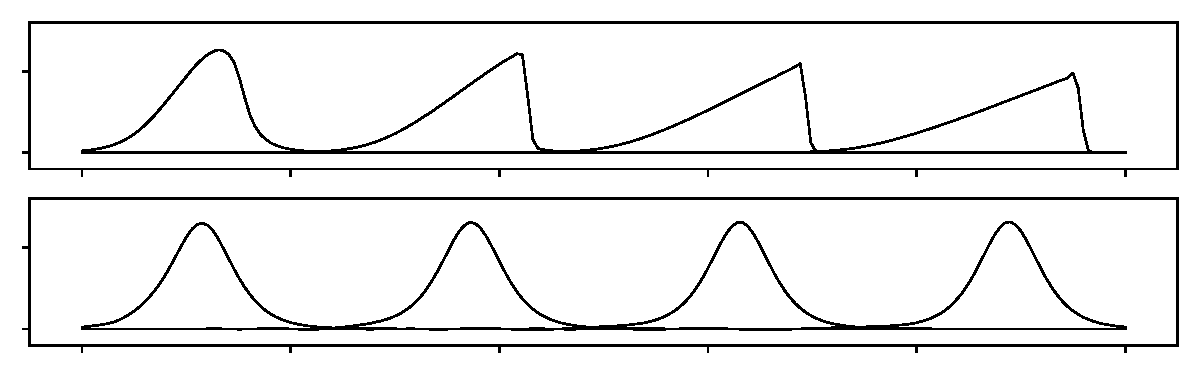
\includegraphics[width=.95\textwidth]{img/eq/boussinesq_dispersion.pdf}
    \caption{Boussinesq equations. Snapshots of a wave propagation. Top: Amplitude dispersion. Bottom: Frequency dispersion}
    \label{boussinesq_dispersion}
\end{figure}


In practice, this phenomenon does not happen. From linear wave theory we know that the celerity depends not only on the water depth, but also on the wavenumber $k=2\pi/\lambda$. This is known as frequency dispersion and this mechanism is missing on the Saint-Venant equations. The introduction of some extra terms leads to the Boussinesq equations, which model the frequency dispersion. Once the frequency dispersion is included, classical soliton waves can be obtained. In a soliton wave, breaking never occurs during the propagation, since the non linear terms are in equilibrium with dispersive terms.



%%%%%%%%%%%%%%%%%%%%%%%%%%%%%%%%%%%%
%%%%%%%%%%%%%%%%%%%%%%%%%%%%%%%%%%%%



\subsection{Derivation of the modified Boussinesq equations}

There are different ways to derive the Boussinesq equations with slightly different results. Nwogu presented a general framework in \cite{nwogu1993}. A three dimensional wave field with free surface elevation $\eta(x_1, x_2, t)$ and water depth at rest $H(x_1, x_2)$ is considered. The fluid is governed by the Navier-Stokes equations but the shallow water assumptions are modified. The fluid is assumed to be incompressible and the flow is assumed to be irrotational. As in the shallow water equations, the vertical velocity is considered to be small, but the vertical acceleration is not negligible. The nonlinearity and dispersion ratios (\ref{nonlin_disp_ratios}) are assumed to be small. The last difference between the shallow water equations and the Boussinesq consist in considering the horizontal velocity at a specified water depth instead of the mean value.

\begin{figure}
    \centering
    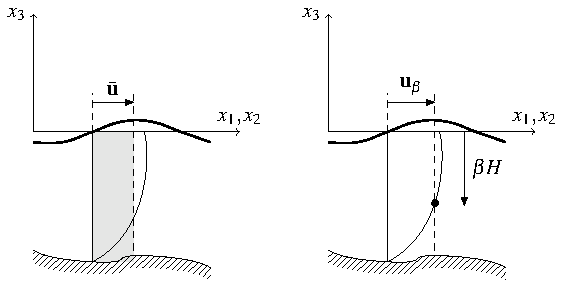
\includegraphics[width=.9\textwidth]{img/eq/velocity_beta.pdf}
    \caption{The modified Boussinesq equations consider the velocity at an arbitrary depth $\beta H$ instead of the mean velocity}
\end{figure}

Finally, the fluid at the free surface has to satisfy a dynamic and kinematic boundary conditions. At the bottom, the fluid has to satisfy a kinematic boundary condition.

\begin{equation}\label{dyn_kyn_bc}
\begin{aligned}
p &= 0 \ , \quad &&\text{at } x_3=\eta \\
u_3 &= \pder{\eta}{t} + u_1 \pder{\eta}{x_1}  + u_2 \pder{\eta}{x_2} \ , \quad &&\text{at } x_3=\eta \\
u_3 &= -u_1 \pder{H}{x_1} -u_2 \pder{H}{x_2} \ , \quad &&\text{at } x_3=-H
\end{aligned}
\end{equation}

Then, the continuity and momentum equations are integrated from the bottom to the free surface and applying the boundary conditions (\ref{dyn_kyn_bc}). Since the average horizontal velocity has been substituted by the velocity at a certain depth, the vertical profile of the velocities must be known. The key of the Boussinesq equations consist in finding an assumption which preserves the the effect of the frequency dispersion. The horizontal velocities $\mathbb{u}=(u_1, u_2)$ are expanded in Taylor series from the seabed ($x_3=-H$),
\begin{multline} \label{seabed_taylor_expansion}
    \mathbf{u}(x_1,x_2,x_3,t) = \mathbf{u}(x_1,x_2,-H,t) + (z+H)\mathbf{u}_3(x_1,x_2,-H,t) \\ + \sfrac{1}{2}(z+H)^2\mathbf{u}_{3,3}(x_1,x_2,-H,t) + \dots
\end{multline}
where the $3$ subscript denotes differentiation with respect to $x_3$.
Finally, the equations are evaluated at an arbitrary depth $x_3=\beta H$ and the set of Boussinesq-type equations are:

\begin{subequations} \label{bsq_eq}
\begin{equation} \label{bsq_eq_mass}
    \pder{\eta}{t} + \nabla \cdot \left((H+\eta)\mathbf{u}_\beta\right) + \nabla \cdot \mathbf{J}_\eta = 0
\end{equation}
\begin{equation} \label{bsq_eq_mom}
    \pder{\mathbf{u}_\beta}{t} + \nabla \eta + (\mathbf{u}_\beta \cdot \nabla) \mathbf{u}_\beta + \mathbf{J}_u = \mathbf{0}
\end{equation}
\end{subequations}
where the auxiliary fields $\mathbf{J}_\eta$ and $\mathbf{J}_u$ introduce the dispersive mechanism and are defined according to the following expressions
\begin{subequations}
\begin{equation}
    {J}_\eta =
        C_1 H^3 \nabla \nabla \cdot \mathbf{u}_\beta +
        C_3 H^2 \nabla \nabla \cdot (H \mathbf{u}_\beta) 
\end{equation}
\begin{equation}
    {J}_u =
        C_2 H^3 \nabla \nabla \cdot \pder{\mathbf{u}_\beta}{t} +
        C_4 H^2 \nabla \nabla \cdot \pder{(H \mathbf{u}_\beta)}{t} 
\end{equation}
\end{subequations}
and the $C_i$ constants depend on the choice of $\beta$
\begin{equation}
    C_1=\frac{1}{2}\left(\beta^2-\frac{1}{3}\right)\ ,
    C_2=\frac{\beta^2}{2}\ ,
    C_3=\beta + \frac{1}{2}\ ,
    C_4=\beta
\end{equation}



%%%%%%%%%%%%%%%%%%%%%%%%%%%%%%%%%%%%%%%%
%%%%%%%%%%%%%%%%%%%%%%%%%%%%%%%%%%%%%%%%



\subsection{Dispersion properties and range of applicability}

This equations present as a free parameter $\beta$ the relative elevation at which the velocity is evaluated. Its value goes from $-1$ at the seabed, to $0$ at the free surface. Since the equations are an approximation of the fully dispersive and nonlinear problem, the parameter $\beta$ is chosen to minimize the errors introduced by the approximation.
In fact, the original Boussinesq equations does no present any dispersive term in the mass balance equation (\ref{bsq_eq_mass}) and correspond to a specific choice of $\beta$.

The parameter $\beta$ is fixed to $-0.531$ in \cite{nwogu1993}. This value has been obtained reducing the equations (\ref{bsq_eq}) to one dimension and flat bottom. Then, a trial function of small amplitude periodic wave of the type
\begin{equation*}
    \eta = a_0 \exp(i(kx-\omega t)) \ , \quad u_\beta = u_0 \exp(i(kx-\omega t))
\end{equation*}
is substituted into (\ref{bsq_eq_mass}) and (\ref{bsq_eq_mom}). After some algebraic manipulation the following expression for the phase speed is obtained:
\begin{equation}
c^2 = \frac{\omega^2}{k^2} = gh
    \left(\frac{
        1-\left(\frac{1}{2}\beta^2 + \beta + \frac{1}{3}\right)(kh)^2
    }{
        1-\left(\frac{1}{2}\beta^2 + \beta\right)(kh)^2
    }\right)
\end{equation}
The relation between the frequency and the wavelength is also known as \emph{dispersion relation}.
By the other hand, the dispersion relation given by the Linear wave theory or Airy theory is given by
\begin{equation}
c^2 = gh \frac{\tanh kh}{kh}
\end{equation}

Finally, the value of $\beta$ has been chosen to minimize the error at the range of applicability. Some other classical values of beta were obtained in \cite{madsen1991,murray1989}. Figure \ref{phase_speed_beta} shows the sensitivity of the phase speed depending on the parameter $\beta$. The shallow water equations, which drop the dispersive terms of equations (\ref{bsq_eq}) are only valid for the shallow water regime ($kh<0.3$). Fixing the free parameter $\beta=-0.531$ extend the range of applicability of the Boussinesq equations to intermediate depths ($kh<3$).

\begin{figure}
    \centering
    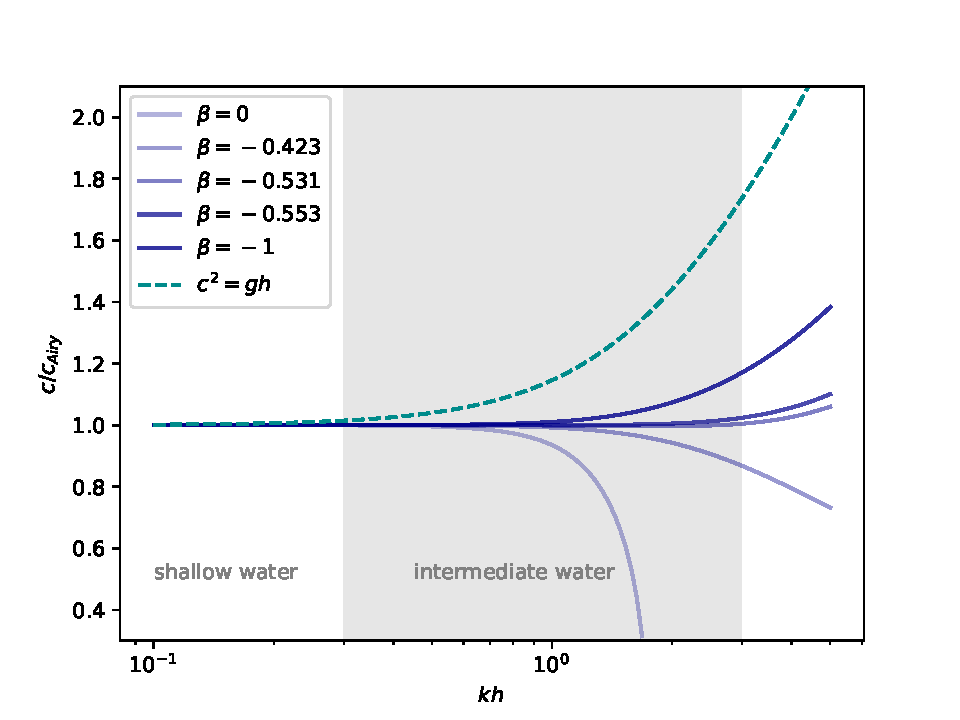
\includegraphics[width=.8\textwidth]{img/eq/dispersion_beta.pdf}
    \caption{Comparison of normalized phase speeds of the Boussinesq modified equations for different values of $\beta$}
    \label{phase_speed_beta}
\end{figure}

According to \cite{ursell1953} the nonlinearity and dispersion parameters $\epsilon$ and $\mu$ can be used for an alternative classification:

\begin{description}
    \item[$\epsilon \ll \mu$]  This configuration correspond to the case where frequency dispersion dominates the problem and linear or Airy theory must be used.
    \item[$\epsilon \sim \mu$] In this case frequency and amplitude dispersion are of the same magnitude and the Boussinesq approximation can be used.
    \item[$\epsilon \gg \mu$] In this situation the amplitude dispersion dominates the problem and the wave will eventually break. This can be simulated using the Saint-Venant or shallow water equations. Since the vertical velocity is assumed negligible, the pressure distribution is assumed to be constant.
\end{description}



%%%%%%%%%%%%%%%%%%%%%%%%%%%%%%%%%%%%%%%%%%%
%%%%%%%%%%%%%%%%%%%%%%%%%%%%%%%%%%%%%%%%%%%



\subsection{Boundary conditions}
\label{equations_bsq_bc}


The boundary conditions presented in section \ref{equations_sw_bc} are applicable to the Boussinesq equations.
However, since the oscillatory behavior is usually prevalent over the convective phenomenon, the boundary conditions are slightly different, both from the physical and the numerical point of view.
The three types of boundary conditions considered for the Boussinesq problems, inflow $\Gamma_I$, reflecting $\Gamma_R$ and absorbing $\Gamma_A$ boundaries have a direct equivalence respectively with the inflow $\Gamma_I$, solid $\Gamma_S$ and outflow $\Gamma_O$ boundaries stated in section \ref{equations_sw_bc}. Those subdomains are such that $\Gamma_I \cup \Gamma_R \cup \Gamma_A = \partial \Omega$, being $\partial\Omega$ the boundary of the domain.

\paragraph{Inflow boundary} Both free surface and velocity are known at $\Gamma_I$. Typically it is used to impose a wave generator. Since the wave amplitude is known, the horizontal velocity can be obtained using linear wave theory.

\paragraph{Reflecting boundary} No fluid should pass through an impermeable wall. This implies imposing the normal component of the velocity to be zero.
\begin{equation*}
    \bar{\mathbf{u}} \cdot \mathbf{n} = 0 \quad \text{on} \ \Gamma_R
\end{equation*}
Following Woo and Liu \cite{woo2004a}, the above relation must be rewritten in terms of $\mathbf{u}_\beta$ and the velocities are related as
\begin{equation*}
    \bar{\mathbf{u}} = \mathbf{u}_\beta + H^{-1} \mathbf{J}_\eta
\end{equation*}
Hence, the complete formulation of a reflective boundary is
\begin{equation}
    \bar{\mathbf{u}}_\beta \cdot \mathbf{n} = 0 \quad
    \mathbf{J}_\eta \cdot \mathbf{n} = 0 \quad
    \text{on} \ \Gamma_R
\end{equation}

\paragraph{Absorbing boundary} An outgoing wave should not return to the computational domain through $\Gamma_A$. A practical implementation of the absorbing boundaries are the sponge layers \cite{israeli1981, wei1995} and will be explained in section \ref{eulerian_bsq_absorbing}





